\documentclass[11pt]{article}


\usepackage[utf8]{inputenc}
\usepackage[T1]{fontenc}
\usepackage{lmodern}
\usepackage{tcolorbox}
\tcbuselibrary{skins}
\usepackage{tikz}

\usepackage{geometry}[scale=0.75]
\setlength{\parindent}{0pt} % Remove indendation after paragraphs

\usepackage{amsmath,amssymb,amsthm}
\usepackage{enumerate}


% -------------------------------------------------
% THEOREM ENVIRONMENTS
% -------------------------------------------------
\theoremstyle{definition}
\newtheorem*{theorem}{Theorem}
\newtheorem*{lemma}{Lemma}
\newtheorem*{proposition}{Proposition}
\newtheorem*{problem}{Problem}
\newtheorem*{corollary}{Corollary}
\newtheorem*{observation}{Observation}
\newtheorem*{definition}{Definition}
\newtheorem*{remark}{Remark}




% -------------------------------------------------
% HYPERREF
% -------------------------------------------------
\usepackage{hyperref}
\hypersetup{
    colorlinks   = true,
    linkcolor    = blue,
    citecolor    = magenta,
    urlcolor     = cyan
}

%% Claim box
\newcounter{claimcount} % Used for proof with lots of claims
\newtcolorbox[use counter=claimcount]{claim}[1][]{%
    colback=green!10, 
    colframe=green!50!black, 
    coltitle=black, 
    fonttitle=\bfseries, 
    boxrule=0.5mm, 
    colbacktitle=green!30,
    enhanced, % Allows additional options
    boxed title style={sharp corners}, 
    attach title to upper={},
    titlerule=0mm, 
    title=Claim: $\;$,
    before=\par\smallskip\noindent, 
    #1
}

%% Equation labelling example for reference

%As for the equations, they’re numbered globally:
%\begin{equation}\label{eq:energy}
%    E = mc^2
%\end{equation}
%Equation~\eqref{eq:energy} is simply (1). The next labeled equation anywhere else in the document will be (2), and so on.

%% End of example

% -------------------------------------------------
% END OF PREAMBLE
% -------------------------------------------------


\begin{document}

\tableofcontents

\newpage

\section{Notation}

I have attempted to introduce all non-standard\footnote{
  That is, non-standard to a student familiar with the A-Level mathematics syllabus. 
} as and when it used, but to save ink here are some is some common notation. If any notation is unclear in this 
document please email me and I'll add it here. 
\begin{itemize}
  \item $\mathbb{N} = \{1, 2, 3, \dots\}$ denotes the positive integers 
  \item $\mathbb{N}_0 = \{0, 1, 2, \dots\}$ denotes the nonnegative integers. 
  \item $\mathbb{Z} = \{\dots, -1, 0, 1, \dots\}$ denotes the integers 
  \item $\mathbb{Q} = \{a/b : a, b \in \mathbb{Z}\}$ denotes the rational numbers 
  \item $\mathbb{R}$ denotes the real numbers, $\mathbb{R}_+$ the positive reals and $\mathbb{R}_{\geq 0}$ the 
  nonnegative reals. 
  \item $\mathbb{C}$ denotes the complex numbers 
  \item $\mathbb{Z}/n\mathbb{Z}$ denotes the integers modulo $n$. 
  \item $\lfloor x \rfloor$ denotes the greatest integer less than or equal to $x \in \mathbb{R}$ 
  \item $\lceil x \rceil$ denotes the smallest integer greater than or equal to $x \in \mathbb{R}$. 
  \item We write $a \mid b$ if $a \in \mathbb{Z}$ divides $b \in \mathbb{Z}$, i.e. if there exists some $k \in \mathbb{Z}$ 
  with $b = ka$. 
  \item $\binom{n}{k} = \frac{n!}{k!(n-k)!}$ denotes the binomial coefficient\footnote{This is sometimes 
  written as $nCr$ and said as ``$n$ choose $k$''. At any reasonable level of mathematical maturity one tends to 
  deviate from this nomenclature and as such, so will we.}.
  \item We use iff on occasion as shorthand for if and only if, or equivalently $\Leftrightarrow$.
  \item $\propto$ denotes proportionality, i.e. $a \propto b$ if there exists $c > 0$ with $a = bc$.
  \item We write $\binom{A}{k}$ to denote the set of subsets size $k$ of $A$. 
  \item We write $\mathcal{P}(A)$ for the set of all subsets of a set $A$.
  \item When clear from context, we use the combinatorial notation $[n] = \{1, \dots, n\}$.
  \item We denote the empty set $\{\}$ by $\emptyset$. 
  \item When defining $a$ to be $b$, we may write $a := b$ to make it clear this is a definition. 
\end{itemize}

\newpage

\section{BMO 1}

\subsection{1999 - 2000}

\subsubsection{Question 2}

\begin{problem}
    Prove that \[2000 \; {\Big |} \; 121^n - 25^n + 1900^n - {(-4)}^n\] 
    for any $n \in \mathbb{N}$
\end{problem}

{\bf Idea: } Factor $2000$ and do some modular arithmetic. 

\begin{proof}[Solution.]

Let \[f: \mathbb{N} \to \mathbb{N}, \; n \mapsto 121^n - 25^n + 1900^n - {(-4)}^n\]
Factor $2000 = 2^4 \cdot 5^3$, then it suffices to prove 
\[5^3 = 125 \; {\Big |} \; f(n) \quad \text{and} \quad 2^4 = 16 \; {\Big |} \; f(n)\]
for each $n \in \mathbb{N}$. These are easily seen working modulo $16$ and $125$. Observe
\[f(n) \equiv 9^n - 9^n + (-4)^n - (-4)^n \equiv 0 \pmod {16}\]
and 
\[f(n) \equiv (-4)^n - 25^n + 25^n - (-4)^n \equiv 0 \pmod {125}\]
Hence, we deduce $2000 \mid f(n)$.
\end{proof}

\begin{remark}
    A competitor not yet familiar with modular arithmetic may prove, for integer $k$ and positive integer $n$,
    \[a \; {\Big |} \; b^n \quad \Longrightarrow \quad a \; {\Big |} \; (b + ka)^n\]
    by using the fact 
    \[a \; {\Big |} \; b \quad \Longrightarrow \quad a \; {\Big |} \; b + ka\]
    and expanding $(b + ka)^n$. All of this is elementary and leads to an analogous solution. 
\end{remark}

\newpage 

\subsubsection{Question 3}

\begin{problem}
Let $ABC$ be a triangle with $\angle BAC = 90^\circ$. Find the point $P$ on the perimeter of $ABC$ such that the 
quantity \[|AP| + |BP| + |CP|\] is minimised.
\end{problem}

{\bf Idea:} Notice an invariant that reduces the problem to three cases. The non-trivial case is to be handled using 
the equality of areas in congruent triangles. 

\begin{proof}[Solution]
    Suppose $P$ is on $BC$. Then it is clear $|BC| = |BP| + |CP|$ and hence we have an invariant. Thus, it suffices 
    to find $P$ on $BC$ such that $|AP|$ is minimised, which is when $AP$ is orthogonal to $BC$. Identical 
    arguments can be made for when $P$ is on $AB$ and (resp. $AC$) to see we have minimality when $CP$ is orthogonal 
    to $AB$ (resp. $BP$ orthogonal to $AC$). \\ 

    {\bf Case 1: $P$ on $BC$}: \\
    $P$ is the foot of the altitude from $A$. Hence the triangle $APB$ is congruent\footnote{By SAS or AAA.} to 
    $APC$. In particular they both have equal area, which allows us to deduce
    \[\frac{|AP| \cdot |BP|}{2} = \frac{|AB| \cdot |AC|}{4} = \frac{|AP| \cdot |CP|}{2} \Longrightarrow 
    |AP| = \frac{|AB| \cdot |AC|}{|BP| + |CP|} = \frac{|AB| \cdot |AC|}{|BC|}\]
    where the implication follows via simple algebra. All together 
    \[|AP| + |BP| + |CP| = \frac{|AB||AC|}{|BC|} + |BC|\]

    {\bf Case 2: $P$ on $AB$} \\
    $AC$ is the altitude from $C$ and has foot $A$. Hence, $P = A$ and
    \[|AP| + |BP| + |CP| = |AB| + |AC|\]

    {\bf Case 3: $P$ on $AC$} \\
    By an identical argument see that, again, $P = A$ and
    \[|AP| + |BP| + |CP| = |AB| + |AC|\]

    Let $|AB| = a$, $|AC| = b$ and $|BC| = c$. Suppose $P = A$, which is the case iff
    \[\frac{ab}{c} + c > a + b\]
    Use the Pythagorean theorem to express
    \[\frac{ab}{c} + c = \sqrt{a^2 + b^2} + \frac{ab}{\sqrt{a^2 + b^2}}\]
    It is equivalent to check\footnote{As the map $x \mapsto x^2$ is monotone increasing on $\mathbb{R}_+$}
    \[\left(\sqrt{a^2 + b^2} + \frac{ab}{\sqrt{a^2 + b^2}}\right)^2 > (a+b)^2\]
    which reduces to 
    \[\frac{a^2b^2}{a^2 + b^2} > 0\]
    and hence it is clear that the original inequality holds everywhere, meaning $P = A$.
\end{proof}

\begin{remark}
    If we didn't spot the invariant, we could've taken a purely coordinate theoretic approach to the problem. This 
    looks ugly, but there could be a nice trick.
\end{remark}

\begin{remark}
    There are many ways we can handle the resulting inequality after our geometry.
\end{remark}

\newpage 

\subsubsection{Question 4}

\begin{problem}
    Define the sequence $(a_n)_{n \geq 0}$ for positive integers $k$ by
    \[a_0 = 1 \quad \text{and} \quad a_n = kn + (-1)^n a_{n-1}, \; n \geq 1\]
    Find all $k$ such that $2000$ is a term in $(a_n)$. 
\end{problem}

{\bf Idea:} Look at the subsequences of even/odd terms of $(a_n)$. This will give us a closed form for $(a_n)$ via 
some bash and it is then a number theory problem. 


\begin{proof}[Solution]
    Run the recursion a second time to see, for $n \geq 2$, 
    \[a_n = kn + (-1)^n \left[k(n-1) + (-1)^{n-1}a_{n-2}\right] = k\left(n + (-1)^n(n-1)\right) - a_{n-2} \tag{$\dagger$}\]
    If the $(-1)^n$ is constant we have easy recursions. Let $(b_n)$ and $(c_n)$ by $b_n = a_{2n}, n \geq 0$ and 
    $c_n = a_{2n+1}, n \geq 0$ respectively. It is clear from $(\dagger)$ that, for $n \geq 1$,
    \[b_n = k(4n-1) - b_{n-1} \quad \text{and} \quad c_n = k - c_{n-1}\]
    Hence we compute
    \begin{align*}
        b_n &= k(4n-1) - b_{n-1} \\ 
        &= k(4n-1) - k(4(n-1)-1) + b_{n-2} \\ 
        &= \cdots \\ 
        &= 4k\sum_{m = 0}^{n-1}(-1)^m (n-m) - k\sum_{r = 0}^{n-1}(-1)^r + (-1)^n 
    \end{align*}
    using $b_0 = a_{2 \cdot 0} = 1$. Similarly, we compute
    \[c_n = k - c_{n-1} = k - k + c_{n-2} = \cdots = k{\bf 1}\{n \text{ odd}\} + (-1)^n (k - 1)\]
    using $c_0 = a_{2 \cdot 0 + 1} = k - 1$, where ${\bf 1}\{\cdot\}$ is the indicator function\footnote{That is, 
    for a subset $A \subseteq \mathbb{N}$ one has ${\bf 1}\{n \in A\} = \begin{cases}1 : n \in A \\ 0 : n \not\in A\end{cases}$}. 
    Now observe, by reversing the order of summation (i.e. by substituting $m \mapsto n-1-m$), 
    \begin{align*}
    &\sum_{m = 0}^{n-1} (-1)^m (n-m) = \sum_{m=1}^{n}(-1)^{n-m} m = (-1)^n \sum_{m=1}^n (-1)^m m \\
    &= (-1)^n \times \left(\underbrace{-1 + 2}_{=1} \underbrace{- 3 + 4}_{=1} \underbrace{- 5 + 6}_{=1}
    - \cdots + (-1)^{n}n\right) = \begin{aligned}\begin{cases} n/2 &: 2 \mid n \\ (n+1)/2 &: 2 \nmid n \end{cases}\end{aligned}
    \end{align*}
    All together, we get 
    \[b_n = \begin{aligned}\begin{cases}1 + 2kn &: n \equiv 0 \pmod 2 \\ 2k(n+1) - k - 1 &: n \equiv 1 \pmod 2\end{cases}\end{aligned}\]
    It is clear that
    \[c_n =  \begin{aligned}\begin{cases} k - 1 &: n \equiv 0 \pmod 2 \\ 1 &: n \equiv 1 \pmod 2\end{cases}\end{aligned}\]
    It suffices to solve $b_n = 2000$ and $c_n = 2000$. For the latter, it is clear only $k=2001$ gives a solution.
    For the former, if $n=2m$, we seek the existence of pairs $(m, k)$ with 
    \[1 + 4km = 2000\]
    By parity, it is immediately clear there are no such pairs. For $n = 2m+1$, solve
    \[k(4m+3) = 2001 = 3 \cdot 23 \cdot 29\]
    Reducing modulo $4$, any solution $(m, k)$ must have $k \equiv 3 \pmod 4$. Hence, writing $k = 3^a 23^b 29^c$ for 
    $a,b,c \in \{0,1\}$, we have $k \in \{3, 23, 3 \cdot 29, 23 \cdot 29\}$. Appending the $k=2001$ solution, 
    obtain \[k \in \{3, 23, 87, 667, 2001\}\]
    as our set of possible $k$.
\end{proof}

\begin{remark}
    It is quicker to list terms, guess the general form of $(a_n)$ and prove it by induction. I jumped straight into 
    computations, hence the inelegance. 
\end{remark}

\begin{remark}
  I wonder if there is a clever trick that allows us to solve without computing a closed-form expression for $a_n$? 
  It doesn't look likely admittedly.
\end{remark}

\newpage

\subsubsection{Question 5}

\begin{problem}
    Suppose there are $7$ people who wish to form $4$ teams to compete in a quiz. In how many ways can they do this? 
    Suppose another person joins, now how many ways can they form the teams?
\end{problem}

{\bf Idea: } Fix the team sizes and count each case. 

\begin{proof}[Solution]
    We will split the count into the cases of possible team sizes. WLOG we fix a descending order on the team sizes. \\

    {\bf Case 1: $(4, 1, 1, 1)$} \\
    Once we've chosen our four person team, there is nothing left to choose. Hence we get $\binom{7}{4} = 35$ 
    combinations. \\ 

    {\bf Case 2: $(3, 2, 1, 1)$} \\
    Once we've chosen our three person team, we have 4 remaining players to choose our two person team from. Hence 
    we get $\binom{7}{3}\binom{4}{2} = 210$ combinations. \\ 
    
    {\bf Case 3: $(2, 2, 2, 1)$} \\
    We choose our two-person teams one after the other as before, but note this time we will count some repetitions. 
    Taking this approach, we count the $3!$ ways of arranging the three two-person teams in a line and hence we have 
    $\binom{7}{2}\binom{5}{2}\binom{3}{2}\frac{1}{3!} = 105$ combinations. \\ 

    Thus, summing over our disjoint possibilities, we obtain $350$ combinations in total. \\ 

    For the second part of this problem we take an essentially identical approach to see that there are $1701$ combinations. 
    This is left to the reader.
\end{proof}

\begin{remark}
    We may instead compute the number of combinations in case 3 as 
    \[\binom{7}{2,2,2} \frac{1}{3!} = \frac{7!}{2!2!2!3!} = 105\] 
\end{remark}

\begin{remark}
    We could also recognise these as the Stirling numbers of the 2nd kind $S(7, 4)$ and $S(8, 4)$. These obey 
    \[S(n+1, k) = kS(n, k) + S(n, k-1)\] which trivialises the second part.
\end{remark}

\newpage

\subsection{2000 - 2001}

\subsubsection{Question 1}

\begin{problem}
    Find all two digit $n \in \mathbb{N}$ for which the digit sum of $10^n - n$ is divisible by $170$. 
\end{problem}

{\bf Idea:} $10^n - n = 99\cdots 9ab$, so count the $9$s and hence compute the digit sum explicitly. 

\begin{proof}[Solution]
    Let $d(m)$ be the digit sum of an integer $m$. Then, 
    \[d(10^n - n) = 9(n-2) + d(100 - n) \tag{$\dagger$}\]
    Write $n = 10x + y$ for some $1 \leq x \leq 9$ and $0 \leq y \leq 9$. We deduce from $(\dagger)$
    \[d(10^n - n) = \begin{aligned}\begin{cases}89x - 8 \; &: \; y = 0 \\ 
    89x + 8y + 1  \; &: \; \text{otherwise}\end{cases}\end{aligned}\]
    If $y = 0$ we check for divisibility by $10$ and see that $x = 2$ is forced, which we can verify gives $n=20$ as 
    a solution. Now, for $y \neq 0$, we first observe 
    \[170 \; {\Big |} \; 89x + 8y +1 \Longrightarrow 89x + 8y \geq 169 \Longrightarrow x \geq 2\]
    Further, by parity, we see that $x$ must be odd. Now we check $x \in \{3, 5, 7, 9\}$ individually. If 
    $n = 10x + y$ is a viable $n$ then
    \[x = 3 \Longrightarrow 170  \; {\Big |} \; 268 + 8y \Longrightarrow y = 9 \tag{1}\]
    \[x = 5 \Longrightarrow 170 \; {\Big |} \; 446 + 8y \Longrightarrow y = 8 \tag{2}\]
    \[x = 7 \Longrightarrow 170 \; {\Big |} \; 624 + 8y \Longrightarrow y = 7 \tag{3}\]
    \[x = 9 \Longrightarrow 170 \; {\Big |} \; 802 + 8y \Longrightarrow y = 6 \tag{4}\]
    Combining (1), (2), (3), (4) and recalling that when $y = 0$ we had $n=20$ forced, our possible solutions 
    can be listed as \underline{$n = 20, 39, 58, 77, 96$}.
\end{proof}

\begin{remark}
    We could've just manually checked each $x \in \{0, 1, \dots, 9\}$, rather than ruling out most of these by 
    parity / bounding, making this problem highly accessible. 
\end{remark}

\newpage 

\subsubsection{Question 3}

\begin{problem}
    A {\it tetromino} is a shape composed of four unit squares, each adjacent to at least one other. 
    \begin{enumerate}[(i)]
        \item Prove there are exactly $7$ tetrominos up to rotation. 
        \item Can we tile\footnote{
          Equivalently, can we pack the $7$ tetronimos into a $4 \times 7$ rectangle such that no two tetronimos 
          overlap?
        } the $7$ tetrominos into a $4 \times 7$ rectangle?
    \end{enumerate}
\end{problem}

{\bf Idea:} (i) fix the maximum number of adjacent squares (ii) colour and spot an invariant

\begin{proof}[Solution to i]
For each tetromino $A$, let $\omega(A)$ be the maximal number of adjacent squares in $T$. It is immediately clear 
$\omega(T) \in \{2,3,4\}$. \\

\underline{$\omega(A) = 4$} \\
Clearly there is only one possibility, the $I$-tetromino. \\

\underline{$\omega(A) = 3$} \\ 
Here we observe three possibilities, the $L$-tetromino, $J$-tetromino or $T$-tetromino. Fix an orientation and 
place $3$ squares in a straight line. There are $\binom{3}{1} = 3$ ways to place the two squares on top, and each 
resulting tetromino uniquely corresponds to a tetromino constructed by placing the remaining square underneath. Hence 
there are $3$ such tetrominos. \\

\underline{$\omega(A) = 2$} \\
Here we observe three possibilities, the $L$-tetromino, $J$-tetromino or $T$-tetromino. Repeat the $\omega(A) = 3$ 
argument. \\

Hence, we count $1 + 3 + 3 = 7$  tetrominos in total. Explicit constructions are given below. \\

%%% Remark: AI generated tikz diagram, suprisingly good at visual reasoning only took prompts. 

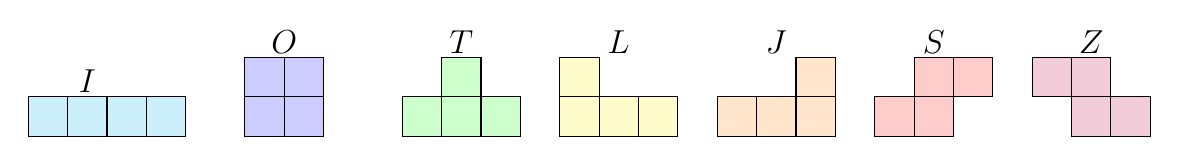
\begin{tikzpicture}[
    scale=0.5,            
    line cap=round,       
    line join=round,      
    every node/.style={   
      font=\large,
      inner sep=1pt
    }
]
\begin{scope}[xshift=0cm, yshift=0cm]
  \foreach \x in {0,...,3} {
    \draw[fill=cyan!20] (\x,0) rectangle (\x+1,1); 
    \draw (\x,0) rectangle (\x+1,1);               
  }
  \node at (1.5,1.4) {$I$};
\end{scope}

\begin{scope}[xshift=5.5cm, yshift=0cm] 
  \foreach \x in {0,1} {
    \foreach \y in {0,1} {
      \draw[fill=blue!20] (\x,\y) rectangle (\x+1,\y+1);
      \draw (\x,\y) rectangle (\x+1,\y+1);
    }
  }
  \node at (1,2.4) {$O$};
\end{scope}

\begin{scope}[xshift=9.5cm, yshift=0cm] 
  \foreach \x in {0,1,2} {
    \draw[fill=green!20] (\x, 0) rectangle (\x+1,1);
    \draw (\x,0) rectangle (\x+1,1);
  }
  \draw[fill=green!20] (1,1) rectangle (2,2);
  \draw (1,1) rectangle (2,2);
  \node at (1.5,2.4) {$T$};
\end{scope}

\begin{scope}[xshift=13.5cm, yshift=0cm]
  \foreach \x in {0,1,2} {
    \draw[fill=yellow!20] (\x, 0) rectangle (\x+1,1);
    \draw (\x, 0) rectangle (\x+1,1);
  }
  \draw[fill=yellow!20] (0,1) rectangle (1,2);
  \draw (0,1) rectangle (1,2);
  \node at (1.5,2.4) {$L$};
\end{scope}

\begin{scope}[xshift=17.5cm, yshift=0cm]
  \foreach \x in {0,1,2} {
    \draw[fill=orange!20] (\x, 0) rectangle (\x+1,1);
    \draw (\x, 0) rectangle (\x+1,1);
  }
  \draw[fill=orange!20] (2,1) rectangle (3,2);
  \draw (2,1) rectangle (3,2);
  \node at (1.5,2.4) {$J$};
\end{scope}

\begin{scope}[xshift=21.5cm, yshift=0cm]
  \draw[fill=red!20] (0,0) rectangle (1,1);
  \draw[fill=red!20] (1,0) rectangle (2,1);
  \draw[fill=red!20] (1,1) rectangle (2,2);
  \draw[fill=red!20] (2,1) rectangle (3,2);

  \draw (0,0) rectangle (1,1);
  \draw (1,0) rectangle (2,1);
  \draw (1,1) rectangle (2,2);
  \draw (2,1) rectangle (3,2);

  \node at (1.5,2.4) {$S$};
\end{scope}

\begin{scope}[xshift=25.5cm, yshift=0cm]
  \draw[fill=purple!20] (0,1) rectangle (1,2);
  \draw[fill=purple!20] (1,1) rectangle (2,2);
  \draw[fill=purple!20] (1,0) rectangle (2,1);
  \draw[fill=purple!20] (2,0) rectangle (3,1);

  \draw (0,1) rectangle (1,2);
  \draw (1,1) rectangle (2,2);
  \draw (1,0) rectangle (2,1);
  \draw (2,0) rectangle (3,1);

  \node at (1.5,2.4) {$Z$};
\end{scope}
\end{tikzpicture}

%%% End of AI generated material

\end{proof}

\begin{proof}[Solution to ii]
  Colour the squares red and blue in an alternating pattern, so that there are an even number of red and an even 
  number of blue squares. Notice the T-tetronimo, no matter where we place it, will contain either $3$ red or $3$ 
  blue squares. The remaining tetronimos all contain $2$ red and $2$ blue squares no matter where we place them. 
  Deduce that any tiling of the tetronimos into the $4 \times 7$ board must contain an odd number of red and blue 
  squares. Hence, we conclude no such tiling exists. 
\end{proof}

\newpage 

\subsubsection{Question 4}

\begin{problem}
  Let $\{x\}$ denote the nearest integer\footnote{We round up the case when $x = a + 0.5, \; a \in \mathbb{Z}$} to 
  $x \in \mathbb{R}$. Define $(a_n)$ by $a_n = n + \{\sqrt{n}\}$. What is the smallest $k \in \mathbb{N}$ such that
  $a_k, a_{k+1}, \dots, a_{k + 2000}$ are consecutive integers?
\end{problem}

{\bf Idea:} Observe this is equivalent to finding the minimal $k$ with $\{\sqrt{k}\} = \{\sqrt{k + 2000}\}$ and do 
some bounding to solve this equation. 

\begin{proof}[Solution]
  We begin by observing $a_{n + i} \geq a_{n} + i$ with equality if and only if $\{\sqrt{n}\} = \{\sqrt{n + i}\}$. 
  Hence it suffices to find the smallest $k$ such that $\{\sqrt{k}\} = \{\sqrt{k + 2000}\}$. We now work by bounding. 
  Firstly, see that $\{\sqrt{k + 2000}\}$ will round up if $\sqrt{k + 2000} \geq \sqrt{k} + 1$, hence we require\footnote{
    Note we may use $x < y \Longleftrightarrow x^2 < y^2$ as both sides are positive and $x \mapsto x^2$ 
    is strictly increasing on $\mathbb{R}_+$
  }
  \[\sqrt{k + 2000} < \sqrt{k} + 1 \Longleftrightarrow k + 2000 < k + 2\sqrt{k} + 1 \Longleftrightarrow 
  \sqrt{k} > \frac{1999}{2} \Longleftrightarrow k > \frac{1999^2}{4}\]
  Now we claim, for $x \in \mathbb{R}$, if $\{\sqrt{x}\} = \{\sqrt{x + 2000}\}$ then $\{\sqrt{y}\} = \{\sqrt{y + 2000}\}$ 
  for all $y \geq x$. One way to see this is to notice $\sqrt{y + 2000} - \sqrt{y}$ is a decreasing function\footnote{
    We can prove this with calculus, the Cauchy-Schwarz inequality or Jensen's inequality.}. 
  Let us consider the critical value $x = \frac{1999^2}{4}$. It is clear $\sqrt{x} = 1999/2$ and hence 
  $\{\sqrt{x}\} = 1000$. Further,
  \[\left\{\sqrt{x + 2000}\right\} = \left\{\sqrt{\frac{1999^2}{4} + 2000}\right\} = 
  \left\{\sqrt{\left(\frac{1999}{2} + 1\right)^2}\right\} = 1001\]
  Unfortunately, these quantities are thus not equal. However, our feasible gap between $\sqrt{x+2000} - \sqrt{x}$ will 
  be strictly less than 1 on $(2001/2, 2001^2/2)$. Hence, we will have $x \geq 2001^2/2$. In the case of equality, we 
  have $\{\sqrt{x}\} = 1001$ and 
  \[\left\{\sqrt{x + 2000}\right\} = \left\{\sqrt{\frac{2001^2}{4} + 2000}\right\} 
  = \left\{\sqrt{\left(\frac{2001}{2} + 1\right)^2 - 2}\right\} = 1001\] 
  Hence, any $k \geq \frac{2001^2}{4}$ works. Take 
  \[k = \left\lceil \frac{2001^2}{4} \right\rceil = \left\lceil \frac{2000^2}{4} + 
  \frac{2 \cdot 2000}{4} + \frac{1}{4}\right\rceil = \left\lceil 1001000 + \frac{1}{4} \right\rceil = 1001001\]
  minimally and the problem is solved.
\end{proof}

\begin{remark}
  I'm not particularly pleased with this solution. We handwave the jump from $x \geq \frac{1999^2}{4}$ to $x \geq 
  \frac{2001^2}{4}$. A rigorous justification is desired. 
\end{remark}

\newpage

\subsubsection{Question 5}

\begin{problem}
  Let $ABC$ be a triangle with side lengths $a, b, c$ and circumcircle $\Gamma$ radius $r$. Prove $ABC$ is 
  right-angled if and only if $a^2 + b^2 + c^2 = 8r^2$. 
\end{problem}

{\bf Idea: } Relate the angles at $A, B$ and $C$ and the radius $R$ using the law of sines. 

\begin{proof}[Solution]
  We begin with the following claim, which for some will be a well known fact. 
  \begin{claim}
    \[\frac{a}{\sin \angle BAC} = \frac{b}{\sin \angle ABC} = \frac{c}{\sin \angle ACB} = 2r\]
  \end{claim}
  \begin{proof}[Proof of claim]
    Let $O$ be the centre of $\Gamma$ and draw the altitude from $O$ to $BC$, letting $D$ be the foot. By the 
    inscribed angle theorem we have $\angle BOC = 2\angle BAC$ and hence, as the triangle $OBC$ is isosceles, 
    $\angle OBC = \angle OCB = 90 - \angle BAC$. Thus, 
    \[r = \frac{|BD|}{\sin \left(90^\circ - \angle OCB\right)} = \frac{|BD|}{\sin \angle BAC} = \frac{a}{2\sin \angle BAC}\]
    Repeating for the altitudes $O$ to $AB$ and $O$ to $AC$ proves our claim.
  \end{proof}
  Using our claim, we see that\footnote{Note we assume, as $\Gamma$ is a circle, $r > 0$ to divide through by $4r^2$.}
  \[a^2 + b^2 + c^2 = 8r^2 \quad \Longleftrightarrow \quad \sin^2 \angle BAC + \sin^2 \angle ABC + \sin^2 \angle ACB = 2\]
  Now the problem reduces to trigonometric bash. Let $\angle BAC = A, \; \angle ABC = B$ and $\angle ACB = C$. Then 
    \begin{align*}
      \cos^2 A + &\cos^2 B + \cos^2 C = \cos^2 A + \cos^2 B + \cos^2 (180^\circ - (A+B)) \\ 
      &= \cos^2 A + \cos^2 B + \cos^2 (A+B) \\ 
      &= \cos^2 A + \cos^2 B + (\cos A \cos B - \sin A \sin B)^2  \\ 
      &= \cos^2 A + \cos^2 B + \cos^2 A \cos^2 B + \sin^2 A \sin^2 B - 2\sin A \sin B \cos A \cos B \\
      &= 1 + \cos^2 A \cos^2 B + (1 - \cos^2 A)(1 - \cos^2 B) - 2\sin A \sin B \cos A \cos B \\ 
      &= 1 + 2\cos^2 A \cos^2 B - 2\sin A \sin B \cos A \cos B \\ 
      &= 1 - 2\cos A \cos B \cos C
    \end{align*} 
  Hence, 
  \[\sin^2 A + \sin ^2 B + \sin^2 C = 2 + 2\cos A \cos B \cos C\]
  Clearly, this is equal to $2$ iff one of $A, B$ or $C$ are equal to $90^\circ$ so we're done.
\end{proof} 

\begin{remark}
  The first claim we made, as with the trig indentity we proved, are fairly well known\footnote{
    Fairly well known in olympiad circles that is, I didn't know them!
  }. If one knows both of these 
  facts the problem is trivial. 
\end{remark}

\newpage

\subsection{2001 - 2002}

\subsubsection{Question 1}

\begin{problem}
  Find all $(m, n) \in \mathbb{N} \times \mathbb{N}$ such that $n$ is odd and \[\frac{1}{m} + \frac{4}{n} = \frac{1}{12}\]
\end{problem}

{\bf Idea:} Rearrange and turn into a divisibility problem. 

\begin{proof}[Solution]
  Observe, 
  \[\frac{1}{m} + \frac{4}{n} = \frac{1}{12} \Longrightarrow 12n + 48m = mn \Longrightarrow (m-12)(n-48) = 12 \cdot 48 = 2^6 3^2\]
  Hence, $m-12 = 2^{a}3^b$ and $n-48 = 2^{6-a}3^{b-2}$ for integer $a,b$. Further, $n$ odd $\Rightarrow a = 6$ so 
  \[(m, n) \in \left\{(588, 49), \; (204, 51), \; (76, 57)\right\}\]
  are the only possible solutions.
\end{proof}

Here is a more obvious solution, taking the natural approach to solve $m = f(n)$. 

\begin{proof}[Alternative solution]
  Observe, by simple algebra, 
  \[\frac{1}{m} + \frac{4}{n} = \frac{1}{12} \Longrightarrow m = \frac{12n}{n-48}\]
  Hence it suffices to solve the equation 
  \[n - 48 \; {\Bigg |} \;  12n \quad \Longrightarrow \quad n - 48 \; {\Bigg |} \;  12n - 12(n - 48) = 576 = 2^6 \times 3^2\]
  Thus, we have $n = 2^a 3^b$ for $a = 0, \dots, 6$ and $b = 0, 1, 2$ and $n$ odd gives $a = 0$. We once again deduce 
  \[(m, n) \in \left\{(588, 49), \; (204, 51), \; (76, 57)\right\}\]
  are the only possible solutions.
\end{proof}

\begin{remark}
  This is one of the rare BMO problems where working iteratively, taking the obvious step each time, does actually 
  work. The less obvious, i,e.~non alternative, does not depend on the knowledge that, for all $k \in \mathbb{Z}$,
  \[a \; {\Big |} \; b \quad  \Longrightarrow \quad a \; {\Big |} \; b - ka\]
  making it accessible to even the most inexperienced candidates. 
\end{remark}

\newpage

\subsubsection{Question 3}

\begin{problem}
  Solve over $x \in \mathbb{R}_+$ the equation 
  \[x + \left\lfloor \frac{x}{6} \right\rfloor = \left\lfloor \frac{x}{2} \right\rfloor + \left\lfloor \frac{2x}{3}\right\rfloor\]
\end{problem}

{\bf Idea:} Reduce to an integer equation and check cases modulo $6$.

\begin{proof}[Solution]
  Observe that the RHS is always in $\mathbb{Z}$, whereas the LHS is in $\mathbb{Z}$ if and only if $x \in \mathbb{Z}$. 
  Hence, it suffices to solve over $x = n \in \mathbb{N}$. To do this, we look at the cases on $n$ modulo $6$. Write 
  $n = 6m + k, k = 0,\dots,5$. Then it is clear our equation reduces to 
  \[k = \left\lfloor \frac{k}{2} \right\rfloor + \left\lfloor \frac{2k}{3} \right\rfloor\]
  which is true if and only if $k \neq 1$. Hence our solution set is 
  \[x \in \mathbb{N} \setminus \{n \in \mathbb{N} : n \equiv 1 \! \! \! \pmod 6\}\]
  and the problem is solved. 
\end{proof}

\begin{remark}
  Boring and easy, I would expect this to be a question 1 on a modern paper.
\end{remark}

\newpage

\subsubsection{Question 4}

\begin{problem}
  Suppose $12$ people are seated around a circular table. In how many ways can $6$ pairs shake hands so that 
  no sets of arms cross?
\end{problem}

\begin{proof}[Solution]

\end{proof}

\newpage

\subsubsection{Question 5}

\begin{problem}
  Let $f: \mathbb{N} \to \mathbb{N}$ be strictly increasing with 
  \[f(n+f(m)) = f(n) + m + 1 \tag{$\dagger$}\]
  for all $m, n \in \mathbb{N}$. What are the possible values of $f(2001)$? 
\end{problem}

{\bf Idea:} Notice $f$ has constant differences and hence is linear. 

\begin{proof}[Solution]
  Substituting $n \mapsto n + 1$ into $(\dagger)$ and taking the difference with $n \mapsto n$, see
  \[f(n + f(m) + 1) - f(n + f(m)) = f(n+1) - f(n) \tag{$\ddagger$}\]
  for all $m, n \in \mathbb{N}$. Hence, a shift by $f(m)$ does not alter the difference $f(n + 1) - f(n)$. We naturally 
  conjecture that $f$ has constant differences. 
  \begin{claim}
    $f(n+k+1) - f(n+k) = f(n+1) - f(n)$ for all $n, k \in \mathbb{N}$.
  \end{claim}
  \begin{proof}[Proof of claim]
    It is clear $f: \mathbb{N} \to \mathbb{N}$ strictly increasing $\Rightarrow f$ unbounded. Hence, we may choose
    $m \in \mathbb{N}$ with $f(m) \leq k < f(m+1)$. Again, using the monotonicty of $f$, see
    \[f(n + f(m)) \leq f(n + k) \leq f(n + f(m + 1))\]
    and 
    \[f(n + f(m) + 1) \leq f(n + k + 1) \leq f(n + f(m + 1) + 1)\]
    Subtracting these inequalities and using $(\ddagger)$, we deduce our claim. 
  \end{proof}
  Our claim makes it clear\footnote{
    To see this, use $f(n+1) - f(n) = c \in \mathbb{N}$ and backwards induct $f(n) = c(n-1) + f(1)$.
  } that $f$ is linear, i.e.~there exist constants $a, b \in \mathbb{Z}$ such that for all $n \in \mathbb{N}$ 
  we have $f(n) = an + b$. Using $(\dagger)$ with $n = m$, observe 
  \[a(n + an + b) + b = an + b + n + 1 \Longleftrightarrow (a^2 - 1)n = 1 - ab\]
  For the LHS to be constant, $a \in \{\pm 1\}$ is forced. $f$ strictly increasing $\Rightarrow a = 1 = b$ so that 
  $f(n) = n + 1$ for all $n \in \mathbb{N}$. We conclude $f(2001) = 2002$ is the only possibility.
\end{proof}

\begin{remark}
  The phrasing of this problem suggests it is possible to do this without solving the functional equation. I 
  cannot see a feasible way. 
\end{remark}

\newpage 

\subsection{2002 - 2003}

\subsubsection{Question 3}

\begin{problem}
  Let $x, y, z \in \mathbb{R}_+$. Given that $x^2 + y^2 + z^2 = 1$, prove 
  \[x^2 yz + xy^2 z + xyz^2 \leq \frac{1}{3}\]
\end{problem}

\begin{proof}[Solution]
  Let $\cdot$ denote the dot product in $\mathbb{R}^3$. By the Cauchy-Schwarz inequality,
  \[x^2 y z + xy^2 z + xyz^2 = (xyz, xyz, xyz) \cdot (x,y,z) \leq \lVert (xyz,xyz,xyz) \rVert \lVert (x,y,z) \rVert 
  = \sqrt{3}xyz\] 
  By the AM-GM inequality, 
  \[\sqrt[3]{x^2y^2z^2} \leq \frac{x^2 + y^2 + z^2}{3} = \frac{1}{3} \Longrightarrow xyz \leq \frac{1}{3\sqrt{3}}\]
  The result immediately follows. 
\end{proof}

\begin{remark}
  There is an elementary solution using only the trivial inequality, but this is far from obvious. See 
  \href{https://math.stackexchange.com/questions/2757796/british-maths-olympiad-bmo-2002-round-1-question-3-proof-without-cauchy-schwar}{the mathematics stack exchange}
\end{remark}

\newpage

\subsubsection{Question 4}

\begin{problem}
  Let $m, n \in \mathbb{N}$ and consider a $m \times n$ grid $R$ of lattice points\footnote{
    That is, points with integer coordinates.
  } in the plane. What is the maximum number of points in $R$ we may colour red so that no collection of $3$ red 
  points form a right-angled triangle with sides parallel to the axis?
\end{problem}

\begin{proof}[Solution]
  Let $\chi_{m, n}$ denote the desired quantity. It is clear we have $\chi_{1, n} = n$ and $\chi_{m, 1} = m$, as 
  we may colour each point in the lines $1 \times n$ and $m \times 1$ without inducing a right-triangle (or in fact, 
  any non-degenerate triangle). Now suppose $m, n \geq 2$ and denote the points in $R$ by 
  $(r_{i, j})_{(i, j) \in [m] \times [n]}$. For fixed $j$, it is clear if we colour $r_{i_1, j}$ and $r_{i_2, j}$ 
  with $i_1 \neq i_2$ we cannot colour any other points in the rows $(r_{i_1, j})_{j \in [n]}, (r_{i_2, j})_{j \in [n]}$ 
  without inducing a right-triangle with sides parallel to the axis. Suppose we have a colouring with two distinct 
  points coloured in two distinct columns. Then it is clear we may only colour at most $m$ of these without inducing 
  a right-triangle with sides parallel to the axis. We can repeat our argument for the rows of $R$ to see, if we have 
  two rows with two distinct points coloured that we may only colour at most $n$ points. We deduce $\chi_{n, m} = 
  \max\{m, n\}$ if we colour at least $2$ distinct points in at least $2$ distinct rows or columns. \\ 

  Instead, suppose there is only one column with at least $2$ distinct coloured points. We can colour $m-1$ of points in 
  this ``colourful'' column and $n-1$ points in the row that isn't coloured in the ``colourful'' row. It is clear 
  this is the best we can do with a colourful column. An analogous argument for a colourful row, giving 
  $\chi_{m, n} = m + n - 2$ in this case. Hence, $\chi_{m, n} = \max\{\max\{m, n\}, m + n - 2\} = m + n -2$. 
\end{proof}

\begin{remark}
  This could probably be written in a better way, but the problem is boring when you spot the ``colourful row'' strategy 
  so I'm leaving it here. The problem where we disclude any right-triangle seems more interesting. I can't find an 
  obvious approach like in this question. Perhaps the pigeonhole principle works. Exercise for the motivated reader!
\end{remark}

\newpage

\subsubsection{Question 5}

\begin{problem}
  Solve over $a, b, c \in \mathbb{N}$ the equation \[a!b! = a! + b! + c! \tag{$(\dagger)$}\]
\end{problem}

{\bf Idea:} Keep bounding things until it all comes together

\begin{proof}[Solution]
  WLOG $a \leq b$. Notice, by factoring the terms containing $a$ or $b$, 
  \[a!b! = a! + b! + c! \Longrightarrow a! - 1 = \frac{c!+1}{b!-1}\]
  Hence, if $(a,b,c)$ forms a solution we must have 
  \[b! - 1 \; {\Big |} \; c! + 1 \Longrightarrow b < c\]
  We also spot immediately that $a \geq 3$ is forced. Now, see that 
  \[a!b! = a! + b! + c! \Longrightarrow b! = 1 + \frac{b!}{a!} + \frac{c!}{a!}\]
  As $a \geq 3$, $b \geq 3$ and hence the LHS is even. For the RHS to be even, it is clear we require at least one 
  of $b \leq a+1$ or $c \leq a+1$ to be true. As $b < c$, we deduce $a \leq b \leq a + 1$. Suppose $a = b$, 
  then \[(a!)^2 - 2a! - c! = 0\] which has integral roots\footnote{
    Over the variable $a$ that is. 
  } only if $\sqrt{1 + c!} \in \mathbb{Z}$. This can only happen if $c! = (m-1)(m+1)$ with $\mathbb{Z} \ni m < c$. 
  We can bound $c! \leq c(c+2)$ for all $c \geq 5$ easily, hence we need only check $c \in \{1,2,3,4\}$. By hand we 
  see only $c = 4$ works. In this case we're left with 
  \[(a!)^2 - 2a! - 4! = 0 \Longrightarrow (a! - 6)(a! + 4) = 0 \Longrightarrow a = 3\]
  Hence, the only solution with $a = b$ is $(a, b, c) = (3, 3, 4)$. Now for $b = a + 1$, see 
  \[a!(a+1)! = a! + (a + 1)! + c! \Longrightarrow (a+1)! = 1 + (a + 1) + c!\]
  Now as $c > a + 1$ the RHS has remainder $1$ when divided by $a+1$, whereas the LHS clearly has remainder $0$. 
  Hence, the only solution to $(\dagger)$ is $(a,b,c) = (3,3,4)$.
\end{proof}

\newpage

\section{BMO 2}

\subsection{1999 - 2000}

\subsubsection{Question 2}

\begin{problem}
  For $x, y, z \in \mathbb{R}_+$, minimise $x^2 + 4xy + 4y^2 + 2z^2$ subject to $xyz = 32$. 
\end{problem}

{\bf Idea:} Apply AM-GM to reduce to one variable and apply AM-GM again to finish. 

\begin{proof}[Solution]
  Let $f(x, y, z) = x^2 + 4xy + 4y^2 + 2z^2$. Notice 
  \[f(x, y, z) = (x + 2y)^2 + 2z^2\]
  By AM-GM we have 
  \[x + 2y \geq 2\sqrt{2xy} \; \text{ with equality iff } x = 2y\]
  and hence, fixing $z$, $f(x,y,z)$ is minimised\footnote{This is as $xyz = 32 \Rightarrow xy = 32/z$ 
  and hence the product on the RHS is fixed. In fact, it is well known (proof also via AM-GM) that the sum of 
  two positive variables $u + v$ with fixed product $uv$ is minimised at $u=v$ so could've instead have just quoted 
  this, though proving things yourself is always preferred!} at $x=2y$. We can thus reduce to
  \[g(y, z) = 16y^2 + 2z^2\]
  Now $xyz = 32 \Rightarrow z = 16/y^2$ so we further reduce to
  \[h(y) = 16y^2 + 2 \cdot \frac{16^2}{y^4}\]
  Applying AM-GM again, we see 
  \[h(y) = 8y^2 + 8y^2 + 2 \cdot \frac{16^2}{y^4} \geq 3(8 \cdot 8 \cdot 2 \cdot 16^2)^{1/3} = 96\]
  with equality iff $8y^2 = 8y^2 = 2 \cdot \frac{16^2}{y^4} \Rightarrow y = 2$. Hence \underline{$96$} is our 
  minimal value and this occurs at the point $(x, y, z) = (4, 2, 4)$.
\end{proof}

\begin{remark}
  When applying the AM-GM inequality we want the RHS to be constant, or we will not be able to deduce the minimal 
  value is at equality. This is why we split into $3$ terms on the second application.
\end{remark}

\begin{remark}
  We could've used calculus to minimise $h(y)$ but calculus + olympiad = bad.
\end{remark}

\newpage 

\subsubsection{Question 3}

\begin{problem}
  Find $a, b \in \mathbb{N}$ with \[(a^{1/3} + b^{1/3} - 1)^2 = 49 + 20 \sqrt[3]{6}\]
\end{problem}

{\bf Idea:} Write $\sqrt{49 + 20\sqrt[3]{6}} = x + y\sqrt[3]{6} + z\sqrt[3]{36}$ for some $x, y, z \in \mathbb{Q}$.

\begin{proof}[Solution] 
  We begin by conjecturing that $\sqrt{49 + 20\sqrt[3]{6}} = x + y\sqrt[3]{6} + z\sqrt[3]{36}$ for some $x, y, z$. This 
  amounts to finding a solution to the system  
  \begin{equation*}
    2xz + y^2 = 0, \; \; 3z^2 + xy = 10, \; \; x^2 + 12yz = 49 
  \end{equation*}
  over $x, y, z \in \mathbb{Z}$. By eliminating variables, we find $(x, y, z) = (-1, 2, 2)$ works. Hence, 
  \[\sqrt{49 + 20\sqrt[3]{6}} = -1 + 2\sqrt[3]{6} + 2\sqrt[3]{36}\]
  To find a solution $(a,b)$ it suffices to solve
  \[a^{1/3} + b^{1/3} - 1 = -1 +2\sqrt[3]{6} + 2\sqrt[3]{36}\]
  It is then clear we may take $a = 48$ and $b = 288$.
\end{proof}

\begin{remark}
  Motivating our conjecture takes some thought. Assuming the existence of\footnote{
    Note the question tells us this exists, so we can cheese our way into this idea. The question ``Are there 
    $a, b \in \mathbb{N}$ with $\dots$? If so, find such a pair.'' would make this idea require a touch more inguinity.}
  such $a, b$, taking square roots tells us $\sqrt[3]{a} + \sqrt[3]{b} - 1 = \sqrt{49 + 20\sqrt[3]{6}}$. If we let 
  $a$ or $b$ be cubes, we see this is doomed. Further, if there does not exist $x \in \mathbb{N}$ with $a = x^3b$ we 
  are also doomed. From here, our conjecture becomes a fairly natural guess. 
\end{remark}


\newpage 

\subsubsection{Question 4}

\begin{problem}
  Find a subset $A \subset \mathbb{N}$ of cardinality $10$ with the property that no $6$ element subset of 
  $A$ has sum divisible by $6$. Can we find $A \subset \mathbb{N}$ of cardinality $11$ with this property? 
\end{problem}

\begin{proof}[Solution] 
  It is sufficient to construct a $10$-tuple $X$ in $(\mathbb{Z}/6\mathbb{Z})^{10}$ with the property that no $6$ 
  elements sum to $0$. Clearly, we cannot have all elements of $X$ being equal\footnote{
    Or we may sum any $6$ of them to obtain $0$.}. 
  We try $2$ unique elements. It suffices to find residues $a, b \in \mathbb{Z}/6\mathbb{Z}$ and multiplicities of 
  $a$ and $b$ respectively $x, y \in \{1, \dots, 10\}, \; x + y = 10$ with our desired property. We need $x=y=5$, or 
  we can sum the same element $6$ times to get sum $0$. We can choose any $a$ and $b$ provided
  $az + b(6-z) \neq 0$ for each $z \in \{1, \dots, 5\}$. By enumeration, we see we can take $a = 1, b = 2$ so that 
  $X = (1,1,1,1,1,2,2,2,2,2)$. We can then take \[A = \{1,7,13,19,25,2,8,14,20,26\}\] to exhibit such a set. \\ 

  A clean proof for the second part is desired. 
\end{proof}

\begin{remark}
  Let $\omega(A)$ denote the number of unique remainders mod $6$ in $A$. It looks like case bashing on
  $\omega(A) \in \{1, 2, \dots, 6\}$ (noticing we can reduce to $\omega(A) \in \{3,4,5\}$ easily) should work, 
  but I can't find a clean proof. You can rule out any case where there are $3$ occurences of the same remainder 
  for example by parity, and I imagine similar arguments rule out the others but I couldn't see them :(
\end{remark}

\begin{remark}
  This is a special case of a theorom of Erd\H{o}s, Ginzburg and Ziv, which states any sequence $a_1, \dots, a_{2m-1}$
  has a subset $I \subset \{1, \dots, 2m-1\}$ of size $m$ with $\sum_{i \in I}a_i \equiv 0 \pmod m$. Proofs of this 
  are highly nontrivial, and mimicking these seems infeasible. The most elementary approach uses the combinatorial 
  Nullstellensatz. 
\end{remark}

\newpage 

\subsection{2000-2001}

\subsubsection{Question 1}

\begin{problem}
  Aegyptus and Brutus initially have $p$ and $q$ marbles respectively, where $p > q$. They take it in turns, starting 
  with Aegyptus, giving each other exactly the number of marbles the other already possesses (e.g. the first turn 
  will be Aegyptus giving Brutus $q$ of his marbles, leaving him with $p-q$ marbles). After $2n$ turns, Aegyptus
  has $q$ marbles and Brutus has $p$ marbles. Find the ratio $\frac{p}{q}$ as a function of $n$. 
\end{problem}

{\bf Idea:} Set up a recurrence relation and solve it.

\begin{proof}[Solution]
  Let $a(n)$ denote the number of marbles Aegyptus has after $n$ turns, where $a(0) := p$. Set $p + q = N$. As 
  Aegyptus moves on turn $2m+1$, we have
  \[a(2m + 1) = a(2m) - (N - a(2m)) = 2a(2m) - N\]
  and, as Brutus moves on turn $2m+2$,
  \[a(2m + 2) = a(2m + 1) + a(2m + 1) = 4a(2m) - 2N\]
  A quick induction\footnote{Work out the first few terms, guess a formula and verify.} shows that, for all $m \geq 0$,
  \[a(2m) = 2^{2m}p - \sum_{k=0}^{m-1}2^{2k} \times (2N)\]
  where $\sum_{\emptyset} \cdots := 0$. We compute, using the well known formula for a geometric series, 
  \[\sum_{k=0}^{m-1}2^{2k} \times (2N) = 2N \frac{2^{2m} - 1}{3}\]
  Hence, 
  \[a(2m) = 2^{2m}p - 2N \frac{2^{2m} - 1}{3}\]
  For our $n$, we know $a(2n) = q$. Thus, letting $x = \frac{p}{q}$, we deduce
  \[q = 2^{2n}p - 2(p + q)\frac{2^{2n} - 1}{3} \Longrightarrow 1 = 2^{2n}x - 2(x + 1)\frac{2^{2n} - 1}{3}\]
  This is a simple linear equation, which can be solved to give 
  \[x = \frac{2 \cdot 4^n + 1}{4^n + 2}\]
  Recalling $x = p/q$ we're done. 
\end{proof}

\newpage 

\subsubsection{Question 2}

\begin{problem}
  Find all $(x, y) \in \mathbb{Z} \times \mathbb{Z}$ with \[1 + x^2y = x^2 + 2xy + 2x + y\]
\end{problem}

\begin{proof}[Solution]
  Observe
  \[1 + x^2 y = x^2 + 2xy + 2x + y \Longrightarrow x \; {\Big |} \; y - 1\]
  by reducing mod $x$. Hence, if $(x, y)$ is a solution there exists $m \in \mathbb{Z}$ with $y = mx + 1$. Hence, 
  by substituting this in and cleaning things up, we see for $x \neq 0$ that
  \[1 + x^2 y = x^2 + 2xy + 2x + y \Longrightarrow m(x^2 - 2x - 1) = 4\]
  Hence, we have $x^2 - 2x - 1 \in \{\pm 1, \pm 2, \pm 4\}$. By checking discriminants we see only the $x$ with
  $x^2 - 2x - 1 \in \{-1, \pm 2\}$ are viable, which yield possible $x \in \{-1, 1, 2, 3\}$. Now, 
  \[1 + x^2 y = x^2 + 2xy + 2x + y \Longrightarrow y = \frac{x^2 + 2x - 1}{x^2 - 2x - 1}\] 
  so we have viable pairs $(x, y) \in \{(-1, -1), (2, -7), (3, 7)\}$. Including the $x = 0$ possibility, we 
  deduce \[(x, y) \in \{(-1, -1), (0, 1), (2, -7), (3, 7)\}\] is our solution set.
\end{proof}

\newpage 

\subsubsection{Question 4}

\begin{problem}
  Suppose there are $n$ dwarves of height $1, 2, \dots, n$ arranged in a circle. Let $V$ denote the sum of the 
  positive differences (i.e.~total variations) between consecutive dwarves. Find the maximum and minimum, 
  over all arrangements of the dwarves, of $V$. 
\end{problem}

{\bf Idea:} For the minimum, consider the arcs with endpoints $1$ and $n$ for each permutation. For the maximum, 
employ a ``centering'' strategy to bound the sum.

\begin{proof}[Solution]
  We claim that the minimum value of $V$ is $2n-2$, which occurs when the dwarves are seated in consecutive order. 
  We also claim the maximum value of $V$ is $\lfloor n^2 / 2 \rfloor$, which occurs when the dwarves are placed in a 
  ``zig-zag'' pattern. \\ 

  Let $\sigma \in S_{n-1}$ be a permutation of $\{1, \dots, n-1\}$ and let $V(\sigma)$ be the total variation of 
  the circle where the dwarf with height $n$ is sat at the head of the table and the dwarf with height $\sigma(i)$ 
  is sat $i \geq 1$ seats along from the head of the table. Let $\text{id}_{n-1} \in S_{n-1}$ denote the identity 
  permutation, which corresponds to the consecutive order seating arrangement. It suffices to see $V(\sigma) \geq 
  V(\text{id}_{n-1})$. \\ 

  It is easy to see $V(\text{id}_{n-1}) = 2n-2$. We have \[V(\sigma) := \sum_{i=1}^{n} |\sigma(i+1) - \sigma(i)|\]
  where $\sigma(n) := n$ is fixed and $\sigma(n+1) = \sigma(1)$ (i.e.~arguments are taking mod $n$). Let us consider 
  the arc $1 = \sigma(i), \sigma(i + 1), \dots, \sigma(i + k) = n$. As each term in the sum is bounded below by $1$, 
  if $k = 1$ it is clear we have $V(\sigma) \geq V(\text{id}_{n-1})$. Otherwise, by the triangle inequality, we have 
  \[V(\sigma) = \sum_{j = 1}^{k} |\sigma(i + j) - \sigma(i + j - 1)| \geq |\sigma(i + k) - \sigma(i)| = n-1\]
  Repeating this argument for the remaining arc we deduce 
  \[V(\sigma) \geq 2(n-1) = V(\text{id}_{n-1})\]
  Now for the maximum, let $f(x) := \left|x - \frac{n+1}{2}\right|$. By the triangle inequality, it is clear that 
  \[\sum_{i=1}^n |\sigma(i+1) - \sigma(i)| \leq \sum_{i=1}^n f(\sigma(i+1)) + f(\sigma(i)) = 2\sum_{i=1}^n f(i) \tag{$(\dagger)$}\]
  We compute $\sum_{i=1}^n f(i)$ for the odd/even cases of $n$. Suppose $n = 2m$, then 
  \begin{align*}
    \sum_{i=1}^{2m} \left|i - \frac{2m+1}{2}\right| &= \sum_{i=1}^m \left|i - \frac{2m+1}{2}\right| 
    + \sum_{i=m+1}^{2m} \left|i - \frac{2m+1}{2}\right| \\ &= \sum_{i=1}^m \left[\frac{2k+1}{2} - i\right] + 
    \sum_{i = m+1}^{2m} \left[i - \frac{2k+1}{2}\right] \\ &= \sum_{i=1}^{2m} i - 2\sum_{i=1}^m i \\
    &= \frac{1}{2}(2m)(2m+1) - 2 \cdot \frac{1}{2}m(m+1) \\ &= m^2
  \end{align*}
  The odd case is similar. For $n = 2m+1$ we compute $\sum_{i=1}^{2m+1} f(i) = m(m+1)$. Hence, using $(\dagger)$, 
  \[V(\sigma) \leq 2 \cdot \left\lfloor \frac{n^2}{4} \right\rfloor = \left\lfloor \frac{n^2}{2} \right\rfloor\]
  We get equality when $|\sigma(i+1) - \sigma(i)| = f(\sigma(i+1)) - f(\sigma(i))$ for all $i \geq 1$, which 
  can be obtained by taking $\sigma(1) = 2, \sigma(2) = n-1, \sigma(3) = 3, \sigma(4) = n-2, \dots, \sigma(n-1) = 1$ 
  in an alternating matter about the midpoint.
\end{proof}

\begin{remark}
  Beautiful problem! I would be interested in seeing alternative approaches.
\end{remark}


\end{document}